\chapter{尾侧前额叶皮层:搜寻目标}
尾侧PF皮层有助于通过显性注意力(眼球运动)和隐性注意力对食物和食物迹象等物体进行视觉搜索,它的连接解释了它如何执行这些功能。尾侧PF皮层,包括额眼区(FEF),与视觉皮层的背侧和腹侧流以及脑干动眼神经核都有联系。明显的注意依赖于它与脑干动眼核的连接,直接或间接地通过上丘和基底神经节。隐蔽注意力依赖于增强的感觉反应,这种反应是通过与视觉皮层以及其他感觉区域的相互作用来调节的。在早期灵长类动物中,随着眶侧PF皮层的颗粒状部分,尾侧PF皮层也在进化(第2章)。这两个新区域一起导致了在精细分支生态位的杂乱环境中发现、关注和评估物体的改进。

\section{介绍}
在前一章中,我们认为眶内PF皮层根据当前的生物需求对物体赋值。本章提出,尾侧前额叶皮层搜索这些物体,它是通过隐蔽地注意周围目标和将眼睛朝向这些目标来实现的。本章的大部分内容都是关于视觉和眼球运动的,它们在脊椎动物历史的早期就已经进化出来了。眼睛和眼外肌肉的证据出现在最古老的脊椎动物和前脊椎动物化石中,有些可以追溯到500多年前(Shu等 2003)。但是灵长类动物在视觉和眼球运动方面有一些重要的创新,比如发展出了中央凹和三色视觉(第2章)。如果我们正确地认为,尾侧PF皮层首先出现在早期灵长类动物身上,那么它比中央凹和全彩视觉都要早:这是关于其功能的重要线索。为了理解尾侧PF皮层,我们首先需要看看它的连接是如何允许灵长类的PF皮层使用眼球运动和隐蔽注意力来搜索食物等物体的。
\section{区域}
在猕猴中,尾侧前额叶皮层指的是位于弓状沟膝侧的皮层。图5.1描绘了它的位置。
% TODO: \usepackage{graphicx} required
\begin{figure}
	\centering
	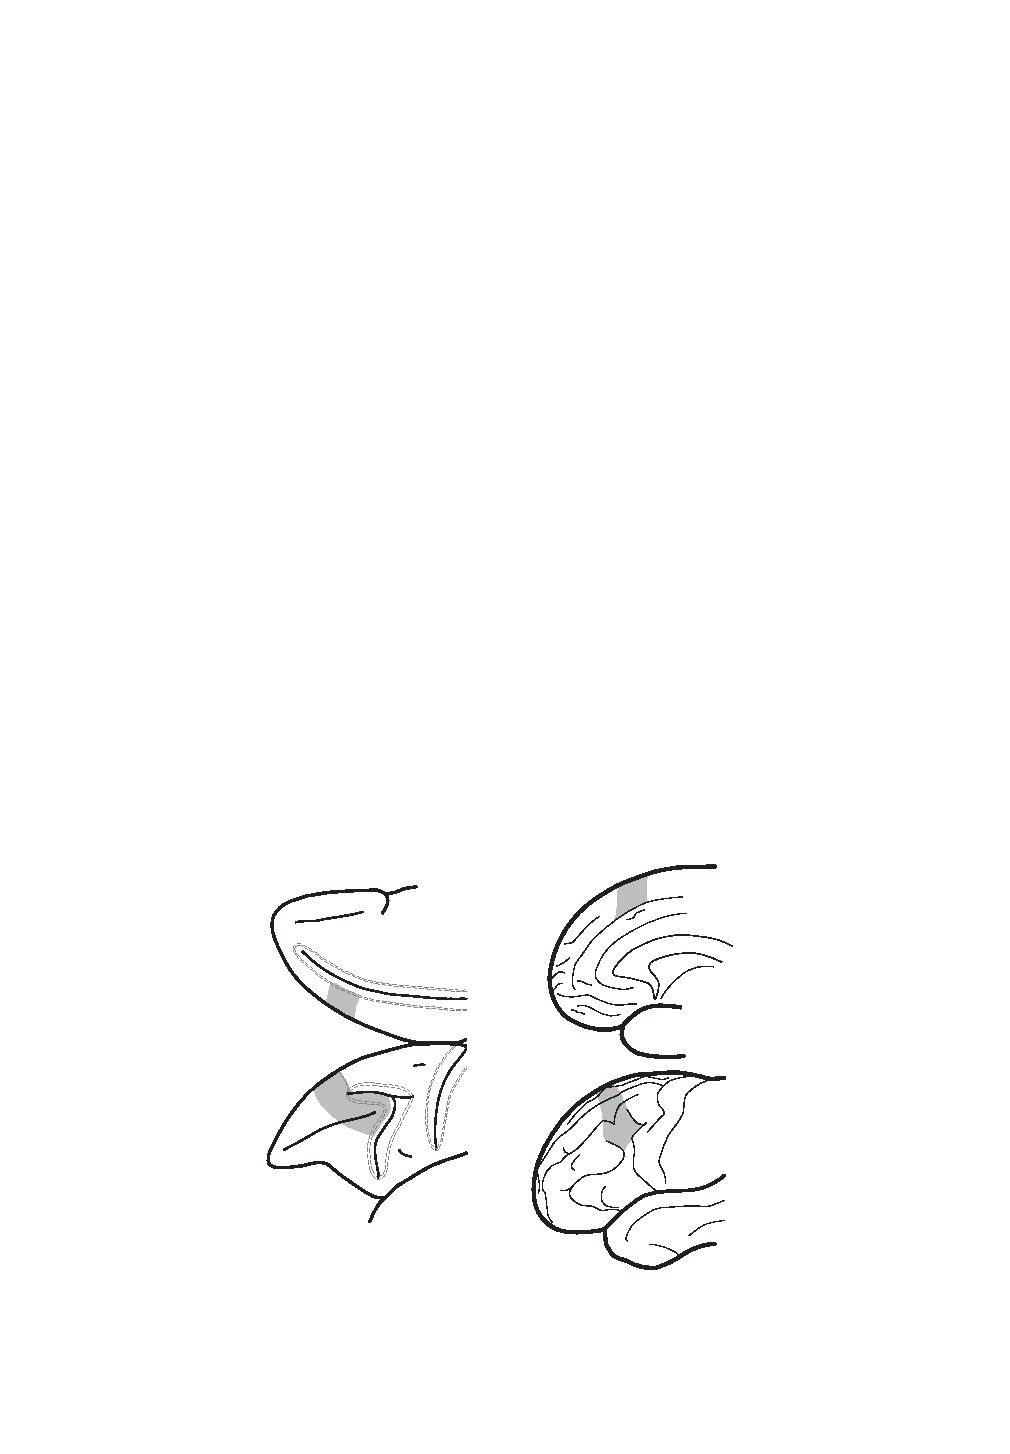
\includegraphics[width=0.7\linewidth]{image_pfc/Fig_5_1}
	\caption{猕猴(左)和人类(右)的尾侧PF皮层。格式如图1.2所示。}
	\label{fig:fig}
\end{figure}

正如我们所定义的那样,尾侧PF皮层总是包括第8区,为了本章的目的,它还包括猕猴主沟的尾侧部分。我们通过注意到,正如在第8区域(Chafee和Goldman-Rakic 1998),主沟尾部的大多数细胞调节其活动与眼球运动相关(Tanila等 1993)来证明这一分组是正确的。Petrides和Pandya(1999)发现了一个位于主沟尾端附近的区域,他们称之为9/46,他们将该区域与相邻的吻侧中外侧PF皮层(46区)和背内侧9区区分开来。顾名思义,Petrides和Pandya认为9/46区具有与9区和46区相似的细胞结构特性,并且这三个区域都具有颗粒状的细胞结构。我们称主沟尾侧皮层为后外侧PF皮层(图1.4),目前将其包括在PF尾侧皮层中。然而,我们承认,在不违反任何解剖学原理的情况下,可以将其包括在PF皮层背侧(第6章)。表1.2使用一个查询标记(“?”)来表示这两个选项。因此,关于后外侧前额叶皮层的许多观点都适用于本章和下一章。

在猕猴中,通过微刺激弓状沟靠近主沟尾端的吻侧岸,可以诱发眼跳运动(Bruce等 1985),这一特性定义了额眼场(FEF)。更高的电流可以通过电流传播,从更大的区域唤起跳视(Robinson和Fuchs 1969),但人们普遍认为低阈值区域对应于FEF。因此,区域8包括FEF,它从典型的颗粒状细胞结构向非颗粒状细胞结构变化(Stanton等 1989)。

Amiez和Petrides(2009)回顾了通过电刺激在人脑中定位FEF的研究。来自中央前上沟吻侧的低阈值刺激,以及来自中央前上沟上方的低阈值刺激,可以诱发眼跳。Amiez等人(2006)使用成像方法来定位与个体受试者皮层解剖相关的激活峰值。FEF,按照这样的定义,始终位于中央前上沟的腹侧分支,这个位置与电刺激所定义的位置大致一致。Amiez和Petrides(2009)提供了猕猴和人类的地图,并表明在这两种情况下,FEF都可以与运动前皮层区分开来,电刺激也可以唤起眼球运动。

微刺激还在猕猴的额叶中发现了第二个眼场:补充眼场(SEF) (Schlag和Schlag- rey 1987)。与FEF一样,SEF中的细胞在扫视前增加活动(Hanes等 1995)。在猕猴中,SEF位于背内侧额叶皮层的第6区(Schlag 和 Schlag- rey 1987;Olson和Gettner 1999),它在人脑中有类似的位置(Amiez和Petrides 2009)。
\section{连接}
图5.2显示了猕猴的尾侧PF皮层的皮质连接,包括FEF。这些数据主要来自Petrides和Pandya(1999),他们将示踪剂注入区域8的细分(区域8B、8Ad或8Av),并描述了它们之间的联系。这项研究比早期的研究更有优势(Petrides和Pandya 1984;Barbas 1988;Barbas 和 Pandya 1989;Cavada和Goldman-Rakic 1989), Petrides和Pandya(1999)进行了小规模和相对选择性的注射。
% TODO: \usepackage{graphicx} required
\begin{figure}
	\centering
	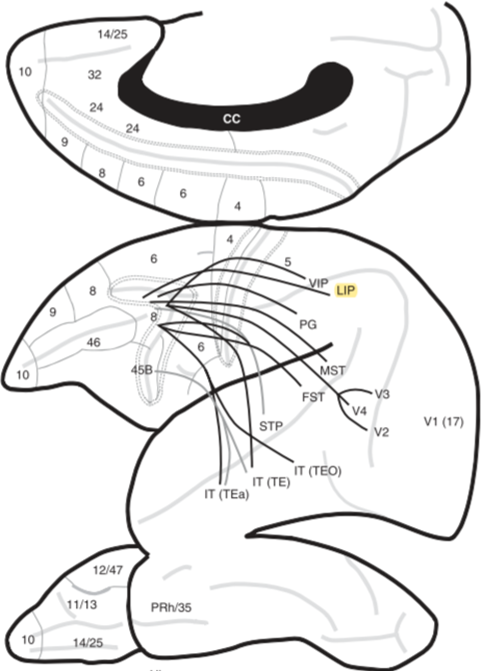
\includegraphics[width=0.7\linewidth]{image_pfc/Fig_5_2}
	\caption{末梢PF皮层的选定连接。图1.4和1.5给出了沟和区域的名称。这些线连接了一些与尾侧PF皮质有轴突直接连接的区域,除非另有说明,假设是相互的。}
	\label{fig:fig}
\end{figure}


根据连接得到以下结论:

\begin{enumerate}
	\item 8Ad区、8B区和后外侧PF皮层与执行眼肌运动和视觉空间功能的区域相连。例如,它们与位于顶骨内沟的LIP区有联系(Cavada和Goldman-Rakic 1989;Andersen等 1990), LIP中的细胞编码眼球运动(Snyder等 1997)。同样的PF区域与下顶叶皮层的PG区域有连接(Cavada和Goldman-Rakic 1989),该区域的许多细胞编码眼睛方向(Sakata等 1980)。最后,8Ad区与颞区MST区有联系,在MST区,细胞对视觉刺激的运动做出反应Celebrini和Newsome 1995)。
	\item 这些视觉区域构成了背侧视觉流的一部分(Ungerleider和Mishkin 1982;Milner和Goodale 2007),以区别于腹侧视觉流。一般来说,背侧流包括后顶叶区域,处理有关动作空间目标的信息,腹侧流包括颞下区域,处理有关视觉刺激的颜色、形状和纹理的信息。
	\item FEF接收早期(低阶)视觉区域的信息,如枕部视觉区V2和V3 (Stanton等 1995),但8Ad区和后外侧PF皮层不接收信息。因此,FEF接收到的高度处理视觉信息比PF皮层尾端的其他部分和PF皮层的其他部分要少。
	\item 8Av区不同于8Ad区、8B区和后外侧PF区,分别与腹侧流和背侧流有联系。8Av区与TEO区有联系(Webster等 1994),也与颞下皮层的其他部分有联系,如颞上沟下岸的皮层(Petrides和Pandya 1999)。
	\item 尾侧PF皮层各组成区域之间相互连接紧密。8Ad区和8Av区彼此相互投射,并与后外侧PF皮层(9/46区)相互投射。这些相互联系支持我们将后外侧皮层纳入本章。如图1.8所示,我们所定义的尾侧PF皮层与Price和Drevets(2010)所定义的尾侧网络非常相似。
\end{enumerate}

图5.2和前面的列表涉及皮质连接,但尾侧PF皮质的皮质连接也解释了其功能的一些重要内容:

\begin{enumerate}
	\item FEF (Künzle, 1976;Huerta等 1986)、8区其余部分(Fries 1984)和后外侧PF皮层(Selemon和Goldman-Rakic 1988)都向上丘发送直接投影。在所有脊椎动物中,上丘及其同源体都有定位头部感受器的功能。因此,这些皮质连接指向了尾侧PF皮层在控制眼球运动方面的作用,但大脑皮层的许多其他部分也投射到上丘(Leichnetz等 1981;Fries 1984),所以这种解剖特征并不能将PF皮层与其他区域区分开来。
	\item FEF还可以通过向基底神经节的投射影响上丘的活动。FEF投射到尾状核的内侧(Stanton等 1988),后者又投射到黑质网状部(Hedreen和DeLong 1991)。该核投射到上丘,在那里发挥抑制作用(Hikosaka和Wurtz 1985)。
	\item 最后,FEF直接投射到脑干动眼肌核(Segraves 1992;Yan等 2001)。
\end{enumerate}

\subsection{总结}
尾侧PF皮层的连接指纹表明,它接受直接的、较低的视觉输入,它具有与背侧和腹侧视觉蒸汽平行的背侧-腹侧区别,并且它通过基底神经节到上丘的投射直接或间接地输出到动眼神经核

\section{FEF是前额叶区域}
尽管有输出表明FEF在控制眼球运动中起作用,但我们并不认为FEF主要在眼球运动控制中起作用。我们知道,当药物抑制FEF时,视觉引导的扫视在被引导到对侧空间时变得不准确(Sommer和Tehovnik 1997)。在这个意义上,FEF类似于运动前皮层。例如,腹侧前运动皮层的失活会导致肢体运动不准确(Kurata和Hoffman 1994)。

我们也知道FEF的永久性损伤不会消除眼跳运动,就像运动前病变不会消除肢体运动一样。然而,一个原因是除了其他区域外,SEF (Huerta和Kaas 1990)和顶叶区域LIP (Holloway 2002)也向上丘发送投影。因此,为了消除眼跳,需要同时去除上丘和FEF (Schiller等 1979,1987)。只剩下最小的扫视。

然而,尽管有这些运动功能的证据,我们认为FEF是前额叶区域,而不是运动前区域。我们这样做是因为我们区分了产生、发现和关注目标的机制和实现目标的机制。记住,我们所说的目标指的是对象或地点,而不是奖励或结果。实现目标的行动会产生结果。除了在实验室,视觉注视和注意力永远不会产生这种意义上的结果。在野外,看着或吃着一种食物并不会产生任何营养或补水的好处。实现这一预期结果需要其他机制。我们认为前者是PF皮层的功能,后者是前运动皮层的范围。

Shadmehr和Wise(2005)在他们对前运动皮层的治疗中提出,它处理的是视运动转换,将伸手运动的视觉目标转换为关节角度和力的变化,从而驱动手到达这些目标。第二章提到了这种机制。详细信息可以在Shadmehr和Wise中找到,但这里有一个简短的总结。

假设有人伸手拿咖啡杯。基本上,电机系统需要建立两个位置:目标位置和手的初始位置。Shadmehr和Wise提出后顶叶和前运动皮层的细胞在一个坐标框架中编码这些位置,在其原点,视觉注视点。然而,在理论上,任何视网膜坐标都可以作为原点。图5.3显示了这种机制是如何工作的。图中显示了两个向量:一个是尾巴在注视点,尖端在运动目标处;另一种是尾巴在固定点,尖端在手的当前位置。两个向量的简单相减就得到了一个向量,它的尾部在手上,顶端在目标上。这个计算的结果相当于一个“运动计划”,将视觉参考系转换为以手为中心的坐标系。前运动区和初级运动区,连同皮层下结构,将这个矢量转换成关节角度的变化和使这个运动的力量。
\begin{figure}
	\centering
	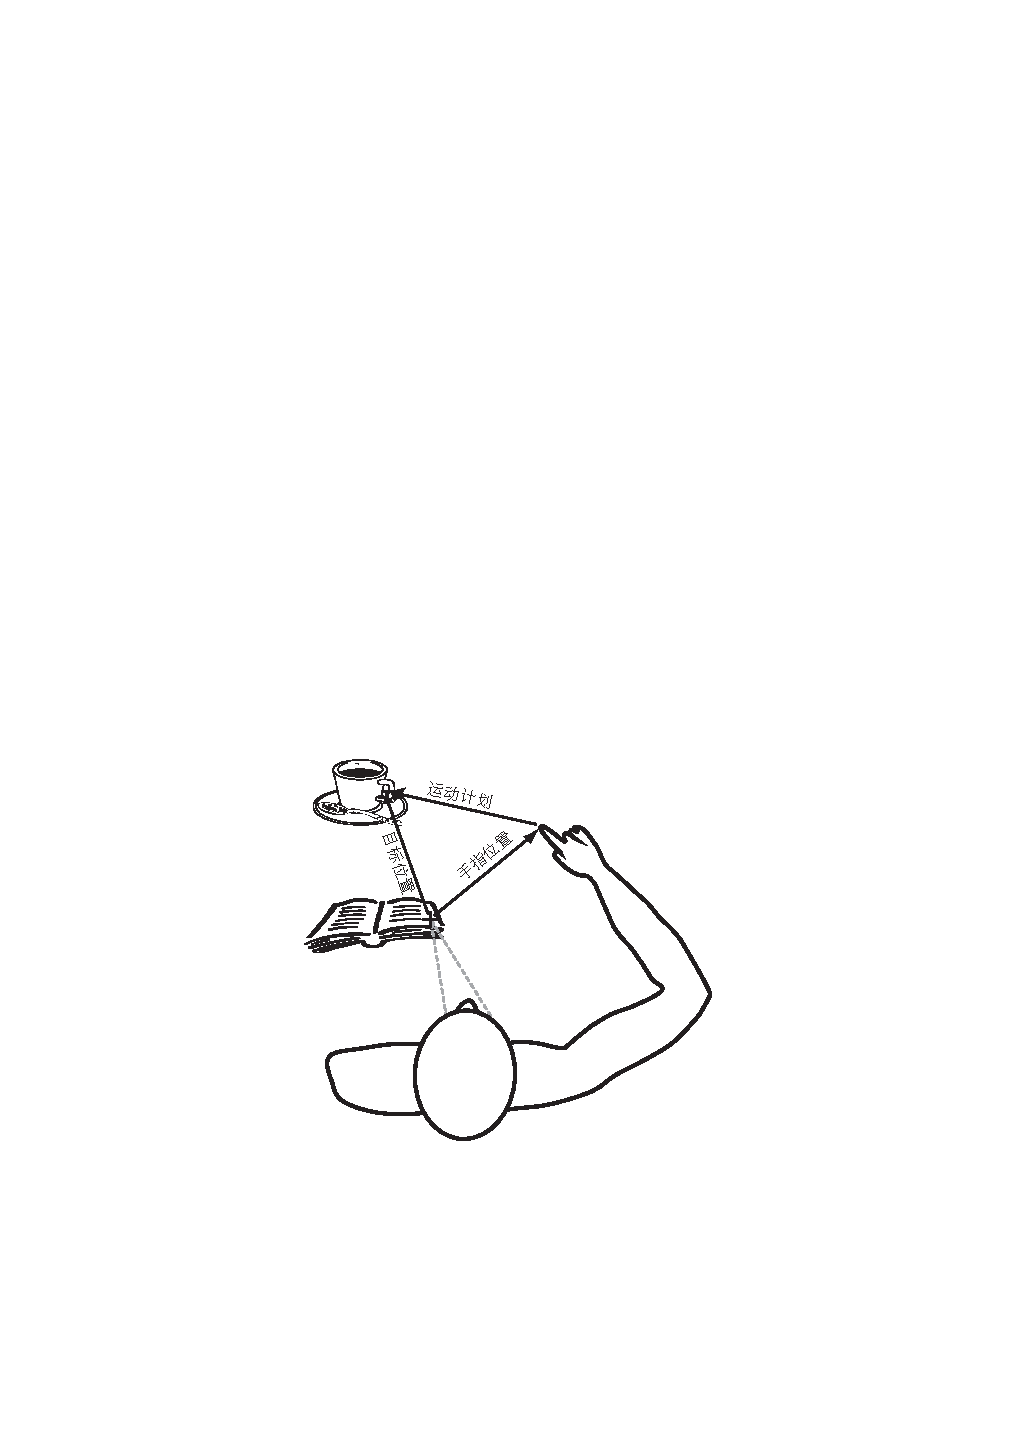
\includegraphics[width=0.7\linewidth]{image_pfc/Fig_5_3}
	\caption{运动平面的矢量表示。这个人的目标是把他的指尖穿过咖啡杯的把手。他或她制定了一个读书计划。+标志着他当时的注视点。来自注视点的两个向量编码目标的位置和手指在非中心的外部坐标框架中的当前位置:注视中心坐标。两个矢量之间的差表示以手为中心坐标的电机平面。修改自Shadmehr R, Wise SP.《触摸和指向的计算神经生物学:运动学习的基础》,©2005麻省理工学院,经麻省理工学院出版社许可。}
	\label{fig:fig}
\end{figure}
通过这种机制或类似的机制,前运动区和后顶叶区以一种眼球运动或其他形式的注意力都无法实现的方式实现目标。在我们的例子中,这个人想要咖啡,所以把他或她的注意力转移到杯子上。注意力可以是显性的,即中央凹朝向杯子,也可以是隐性的,即只关注杯子而不看它。杯子里的东西与人当前的需求有关,因此他或她产生了一个目标——咖啡杯——然后搜索并将注意力转移到杯子上。我们认为,尾侧PF皮层执行搜索和注意功能。虽然视觉固定和注意力不能达到预期的结果,但伸手到杯子里,把它送到嘴里,从里面喝水就可以了。我们将后一种功能视为前运动区和初级运动区,以及运动系统的其他部分。

那么,有什么证据表明FEF参与了对目标的寻找和关注,而不是实现目标的手段?我们已经看到,与运动前区域不同,FEF接收来自低阶视觉区域的直接输入,特别是枕叶和颞叶皮层称为V2、V3、V4和MST的区域(Stanton等 1995)。这些联系解释了为什么FEF中的一些细胞在感觉刺激出现后表现出活动增加,而在运动之前却没有(Schall 1991)。它们似乎明确了视觉目标,而不是注视这些目标所需的眼球运动。此外,在顶叶区LIP投射到FEF的细胞中,78\%有视觉反应,但没有扫视相关活动(Ferraina等 2002)。这种投影可以提供另一种关于视觉目标的信息来源,而且是独立于运动指令的信息来源。

当然,FEF中的许多细胞具有视觉运动活动:它们在视觉目标出现时和眼球运动之前调节自己的活动(Schall 1991)。其中很多都是在刺激出现后不久,即刺激引起注意时,指定刺激的位置。Sato和Schall(2003)教猴子在一系列干扰物中发现一个视觉弹出刺激,然后对该位置进行扫视(prosaccade试验)或对相反方向的扫视目标进行扫视(反扫视试验)。如果活动反映了刺激的位置,那么两种试验类型的活动应该是相同的。

Sato和Schall比较了两项任务中FEF细胞的活动,当弹出的刺激落入细胞的接受野时。对于反眼跳任务,注意当弹出刺激这样做时,眼跳目标是在相反的方向。然而,57\%的任务相关细胞的活动最初反映了刺激的位置,尽管随后86\%的这些细胞后来编码为扫视目标。

这些结果表明,FEF中的细胞活动可以反映刺激的位置,独立于运动,并且这种活动反映了隐蔽注意的方向。与这一观点一致,Armstrong和Moore(2007)表明,FEF的皮质内微刺激增强了视觉区V4(腹侧视觉流的中层区域)的细胞反应。它是专门为视觉空间的一个特定部分做的。刺激FEF的效果可能模仿了猴子在该位置秘密关注物体时所发生的情况。

如果FEF真的在隐性注意和显性注意中起作用,该区域的暂时失活应该会导致对中央凹外刺激的注意受损。因此,Wardak等(2004)教猴子在干扰物中发现目标,而动物则保持对中心光点的固定。在FEF失活后,猴子发现周围目标的速度很慢。Iba和Sawaguchi(2003)表明,失活也会导致猴子对目标进行扫视的速度变慢。这些发现表明,FEF在对刺激的公开注意和隐蔽注意中都有作用,特别是当这些刺激作为后续行动的目标时。

这一观点与第二章中关于前额叶进化的描述非常吻合。Strepsirrhine灵长类动物没有中央凹,早期灵长类动物可能也没有。因为包括FEF在内的尾侧PF皮层在早期灵长类动物中进化而来,它一开始不可能与中央凹或中央凹有任何关系。所以,从这个意义上说,这些动物的所有视觉都对应于中央凹外视觉,所有的注意力都是隐蔽的。顺畅的眼球运动可以让类人猿灵长类动物锁定中央凹,将注意力集中在移动的物体上,并保持高分辨率图像。但这种能力也可能在缺乏中央凹的灵长类动物中进化而来(Shepherd和Platt 2010)。因此,从中央凹视觉或明显的注意力来解释灵长类动物的前额叶皮质的起源是错误的,尤其是尾前额叶皮质的起源。

然而,中央凹最终在后来的灵长类动物中进化出来,现代眼镜猴、猴子、猿和人类(单足纲)通过遗传拥有它。尽管有很多优点,但集中注意力的能力是有代价的。那视觉世界的其余部分呢?这个混乱的世界还包含许多其他突出的项目。在某种意义上,没有中央凹的视网膜提供了一个更平衡的世界观。即使在中央凹进化之后,保持隐蔽注意力的好处是,它可以增强对有限数量的中央凹外物体的处理,即使最密集的处理是用于中心凹的物体和地方。隐蔽注意力和搜索的重要性在于,所有被关注的对象,而不仅仅是被聚焦的对象,都可能成为未来行动的目标。根据这一观点,包括FEF在内的尾侧PF皮层进化为隐蔽的搜索和注意力,但后来一旦中央凹出现,就适应了公开的注意力。
\subsection{总结}
许多神经科学家将FEF视为眼球运动区域,并将其视为眼球运动的前运动区域。我们提出一个不同的想法。我们将FEF和尾侧PF皮层的其他部分视为前额叶区域,而不是运动前区域,并提出它们在寻找和关注灵长类动物重要目标方面发挥作用。在许多灵长类动物中,包括猴子和人类,对目标的关注通常意味着眼球运动,使中央凹朝向目标(扫视)或在目标移动时保持视觉固定(平稳追求)。但是隐蔽的注意力也扮演着重要的角色,在缺乏中央凹的早期灵长类动物中,它肯定是这样的。由于注视是注意力的一种形式,我们将眼球运动视为一种注意力功能,而不是一种运动功能。我们提出,包括FEF在内的尾侧前额叶皮层的功能是将公开或隐蔽的注意力引向一个目标,而不是作为实现目标的机制的一部分。

\section{动眼肌延迟反应任务}
我们将FEF与PF尾部皮层的其余部分分开处理,因为FEF的皮质内微刺激会引起眼球运动。但是,正如在连接部分所解释的那样,FEF与尾侧PF皮层的其他部分有紧密的连接。因此,8区(Chafee和Goldman-Rakic 1998)和后外侧PF皮层(Funahashi et al. 1989)的许多细胞具有与眼球运动相关的活动。

正如我们前面所说的,后外侧PF皮层的连接使我们在本章中将其与包括FEF在内的后外侧PF区一起考虑。我们在第2章中对皮层进化的讨论为这种方法提供了一些可信度,后外侧PF皮层中存在编码眼球运动的细胞。由于后外侧前额叶皮层(9/46区)处于中间状态,在本节中,我们将讨论在第6章中再次出现的主题,最显著的是被称为“空间记忆任务”的任务中的延迟期活动问题。我们这样做主要是为了方便,并认为没有什么关键取决于我们是否将后外侧PF皮层与PF区的尾侧组或背侧组进行分类。

动眼力延迟反应任务在包括后外侧PF皮层在内的尾侧PF皮层的研究中发挥了突出作用。它不同于经典的延迟反应任务,因为猴子通过扫视而不是到达一个空间目标来选择潜在的目标。

动眼肌延迟反应任务有三个阶段:提示、延迟和选择(图5.4)。在第一阶段,一个视觉空间线索会短暂地出现在受试者视野的某个地方。这个刺激指示了猴子必须扫视的位置,但直到延迟期结束,猴子必须继续盯着一个中心光点。在一段从几百毫秒到几秒不等的延迟时间后,一个“开始”信号告诉受试者将扫视移动到最近提示的位置。如果被试的扫视准确,就会得到奖励。

尽管实验人员可以使用任何提示位置的配置,但常见的版本包括以注视点为中心等距排列的八个显著位置,如图5.4所示。该图将位置显示为空方格,并表示球杆为填充方格。然而,重要的是要注意,正如通常所呈现的那样,外围位置没有以任何方式标记,这意味着当猴子响应“go”信号时,它会扫视到屏幕上未标记的位置。

在这项任务中,尾侧和后外侧前额叶的许多细胞表现出延迟期活动(Chafee和Goldman-Rakic 1998)。图5.4显示了Lebedev等人(2004)在种群水平上从尾侧PF皮层记录的记忆信号。

\begin{figure}
	\centering
	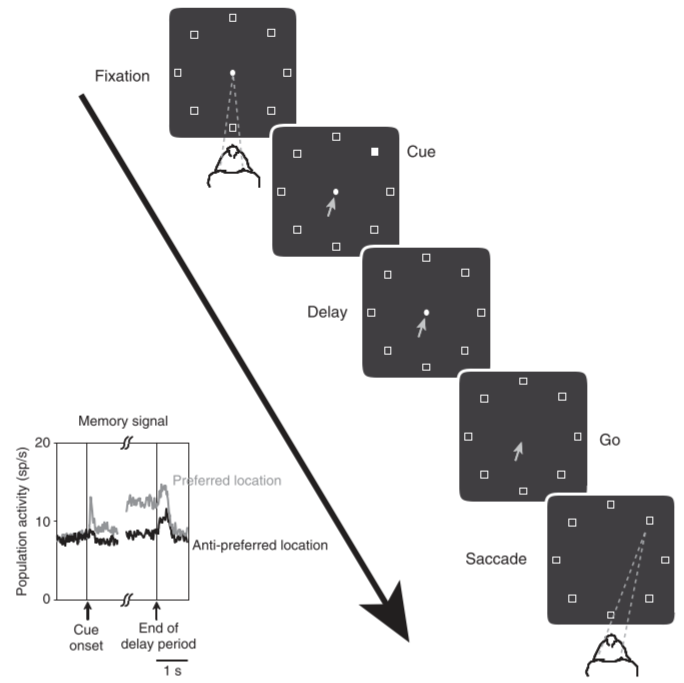
\includegraphics[width=0.7\linewidth]{image_pfc/Fig_5_4}
	\caption{普通版本的动眼器延迟反应任务。在试验过程中,每个面板在不同的时间显示屏幕,在其他试验中,未填充的白色方块是潜在的空间目标。填满的白色方块表示一个例子试验的线索,填满的白色圆圈表示注视点。灰色虚线和灰色箭头表示猴子的注视点。左下方的插入图显示了空间记忆信号,由Lebedev等人(2004)从PF皮层细胞群中记录,灰色为首选记忆位置的平均活动,黑色为反首选位置的平均活动。因为Lebedev等人控制了注意力,这些数据代表了PF皮层空间记忆信号的最有力证据,尽管它们只出现在延迟期间编码位置的少数细胞中。}
	\label{fig:fig}
\end{figure}

Funahashi和他的同事(Funahashi et al. 1989;Takeda和Funahashi 2002)展示了他们的电极穿透皮层的位置图,我们假设这些细胞延伸到整个采样区域。Lebedev等人的研究表明,具有记忆特异性信号的细胞位于主沟尾端9毫米处,主要位于主沟背侧及其附近。Chafee和Goldman-Rakic(1998)报告说,延迟期活动主要来自8A区,但他们的图表显示,一些细胞也来自后外侧PF皮层。

成像实验在类似领域也得到了结果。Inoue et al.(2004)比较了眼肌运动延迟反应任务中的眼跳激活与猴子对屏幕上标记的位置进行眼跳的任务中的激活。差异激活位于后外侧PF皮层和8区,包括FEF。

鉴于以下事实,这是一个重要的观察,下一章将解释,在经典的、达到版本的延迟反应任务上的表现取决于中外侧PF皮层,而不是尾侧PF皮层。因此,动眼肌延迟反应任务不同于经典的延迟反应任务,基于动眼肌版本任务的结论不一定适用于经典的延迟反应或延迟交替任务。后外侧前额叶损伤对这些任务的经典版本缺乏影响(Butters和Pandya 1969),这强化了这样一种观点,即该区域在目标的寻找和关注中发挥作用,而不是在目标的实现(前运动皮层功能)或目标的产生(背侧前额叶皮层功能,如第6章所述)。